\documentclass{article}

\usepackage{arxiv}

\usepackage[utf8]{inputenc} % allow utf-8 input
\usepackage[T1]{fontenc}    % use 8-bit T1 fonts
\usepackage{hyperref}       % hyperlinks
\usepackage{url}            % simple URL typesetting
\usepackage{booktabs}       % professional-quality tables
\usepackage{amsfonts}       % blackboard math symbols
\usepackage{nicefrac}       % compact symbols for 1/2, etc.
\usepackage{microtype}      % microtypography
\usepackage{lipsum}		% Can be removed after putting your text content
\usepackage{graphicx}
\usepackage{natbib}
\usepackage{doi}

\usepackage[english,polish]{babel}
\usepackage{placeins}
\graphicspath{{images/}}


\title{Detekcja zajętości miejsc parkingowych z~wykorzystaniem YOLOv3}

%\date{September 9, 1985}	% Here you can change the date presented in the paper title
%\date{} 					% Or removing it

\author{
    Jakub Motyka \\
	Wydział Elektroniki i Technik Informacyjnych \\
	Politechnika Warszawska \\
	Warszawa \\
	\texttt{jakub.motyka2.stud@pw.edu.pl} \\
	%% examples of more authors
	\And
    Dawid Sygocki \\
	Wydział Elektroniki i Technik Informacyjnych \\
	Politechnika Warszawska \\
	Warszawa \\
	\texttt{dawid.sygocki.stud@pw.edu.pl}
}

\renewcommand{\shorttitle}{Detekcja zajętości miejsc parkingowych}

\hypersetup{
    pdftitle={Detekcja zajętości miejsc parkingowych z wykorzystaniem YOLOv3},
    pdfauthor={Jakub Motyka, Dawid Sygocki},
    pdfkeywords={Detekcja obiektów, YOLOv3, Miejsca parkingowe, PANet},
}

\begin{document}
\maketitle

% keywords can be removed
\keywords{Detekcja obiektów \and YOLOv3 \and Miejsca parkingowe \and PANet}

\section{Wprowadzenie}

Nasz projekt skupia się na wykrywaniu zajętości miejsc parkingowych. W klasycznej odsłonie ten powszechny problem wymagał dedykowanych rozwiązań takich jak bramki biletowe lub czujniki w miejscach parkowania. Nowym rozwiązaniem pojawiającym się na rynku jest wykorzystanie do analizy materiału kamer CCTV głębokich sieci neuronowych. Oznacza to oszczędność: kamery takie często są już i tak zainstalowane w celu zapewnienia bezpieczeństwa

Zdecydowaliśmy się na implementację sieci w architekturze YOLOv3 \citep{redmon2018yolov3}. Jest to sieć jednoprzebiegowa (tj. wykrywająca obiekty bez wcześniejszej predykcji obszarów zainteresowań) cechująca się dobrym stosunkiem jakości wyników do szybkości uczenia i działania.

\section{Zbiór danych}

Do uczenia i testowania modelu wykorzystaliśmy zbiór danych PKLot \citep{de2015pklot} -- jeden z najpopularniejszych zbiorów etykietowanych zdjęć miejsc parkingowych.

Zbiór zawiera 12'416 obrazów w formacie JPEG o wymiarach 1280x720. Pochodzą one z trzech kamer, z czego dwie zamontowane były w obrębie tego samego parkingu, ale prezentują go z różnych perspektyw. Zdjęcia przedstawiają różne warunki oświetleniowe i~atmosferyczne oraz, oczywiście, różny stopień zajętości miejsc.

W skład zbioru PKLot wchodzi łącznie 695'851 etykiet w formacie XML, z czego 48,5\% to miejsca zajęte.

Liczba finalnie używanych obrazów to 12'142, co wynika z błędów w etykietach. Obrazy są odrzucane, jeżeli nie zawierają co najmniej jednej prawidłowej adnotacji. Etykiety przetwarzane są do formatu Pascal VOC, który opisuje każdy prostokąt jako współrzędne środka, szerokość, wysokość oraz klasę, a następnie są one zapisane pod tą samą nazwą co obraz, lecz z innym rozszerzeniem. Pozwala to na szybkie wczytanie obrazów zakwalifikowanych jako poprawne i uzyskanie z nich danych potrzebnych do uczenia.

Dane nie były podzielone na zbiór uczący, walidacyjny i testowy, dlatego dokonaliśmy takiego podziału samodzielnie w stosunku 8:1:1 za pomocą funkcji \texttt{random\_split}. Obecny podział jest losowy.

\section{Analiza literatury}

Przegląd literatury pomógł nam w wyborze architektury sieci, zbioru danych oraz metryki pozwalającej określić jakość rozwiązania. Istotne z naszego punktu widzenia artykuły przedstawione są pokrótce poniżej:

\begin{itemize}
    \item \citep{lisboa2022systematic} stanowi systematyczny przegląd zagadnienia detekcji miejsc parkingowych, podsumowując technologie i zbiory danych wykorzystywane w istniejących pracach oraz porównując otrzymane wyniki,
    \item \citep{ding2019vehicle} rozszerza sieć YOLOv3 o czwarty poziom skali cech (7x7 dla wejścia o rozmiarze 448x448); wykorzystany zbiór danych to podzbiór PKLot -- PUCPR; ramki kotwiczne (\textit{anchor boxes}) zostały dopasowane do zbioru danych za pomocą algorytmu centroidów,
    \item \citep{nguyenyolo5pklot} porównuje wyniki różnych wariantów YOLOv5 na pełnym zbiorze PKLot, uzyskując mAP na poziomie 99,6-99,7\%; w porównaniu wskazane są również inne prace wykorzystujące sieci YOLOv3, Faster R-CNN i Mask R-CNN.
\end{itemize}

\subsection{Projekty wzorcowe}

Implementując sieć YOLOv3, bazowaliśmy na następujących istniejących projektach:

\begin{itemize}
    \item \citep{redmon2018yolov3} (oryginalna implementacja twórcy YOLOv3),
    \item \citep{websiteyolo},
    \item \citep{yolopytorch}.
\end{itemize}

\section{Implementacja podstawowa (\textit{baseline})}

W ramach projektu dokonaliśmy implementacji standardowej sieci YOLOv3 dla wejścia o rozmiarze 416x416 z~użyciem języka Python, bibliotek uczenia maszynowego: PyTorch, PyTorch Lightning i pomocniczych bibliotek do obliczeń i wizualizacji: NumPy, PIL, MatPlotLib.

Procedurą uczenia objęliśmy tylko szyjkę i głowice detekcyjne modelu. W kręgosłupie sieci wykorzystaliśmy wagi uzyskane w ramach treningu na zbiorze ImageNet (dostarczone przez autora YOLOv3 \citep{redmon2018yolov3}).

Zachowaliśmy zgodność wszelkich hiperparametrów z wzorcową optymalizacją.

\subsection{Omówienie architektury}

Bardzo uogólniony schemat YOLOv3 przedstawiony jest na rysunku \ref{fig:simple_yolov3}. Model składa się z kręgosłupa (Darknet53), szyjki (FPN) oraz 3 głowic do detekcji (YOLOv3).

\begin{figure}[!h]
    \centering 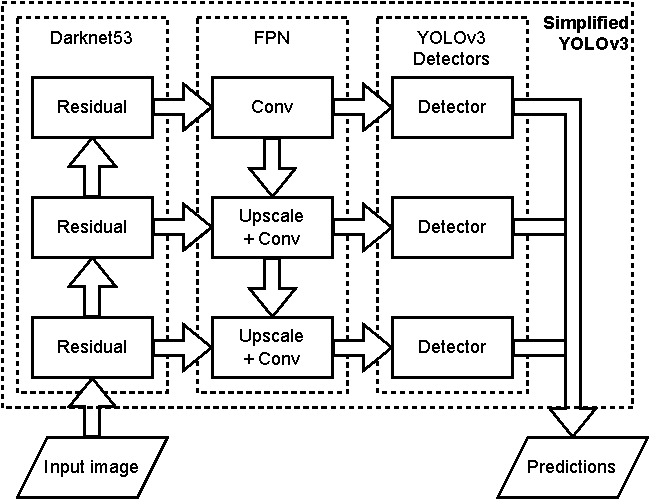
\includegraphics[width=0.6\linewidth]{simple-yolov3}
    \caption{Bardzo uproszczony diagram architektury modelu detekcji obiektów YOLOv3}
    \label{fig:simple_yolov3}
\end{figure}

\paragraph{Warstwa kręgosłupa} (rysunek \ref{fig:darknet}) odpowiada za ekstrakcję cech z obrazu wejściowego. Korzystamy z 3 wyjść kręgosłupa, aby wykorzystać przydatne cechy w różnych rozdzielczościach, a więc i o różnym stopniu przetworzenia.

\paragraph{Szyjka modelu} (rysunek \ref{fig:fpn}) pozwala na propagację cech z późniejszych warstw do wcześniejszych poprzez skalowanie w górę cech o mniejszej rozdzielczości i ich konkatenacje z mniej bogatymi cechami o wyższej rozdzielczości. Finalnie cechy o 3 rozdzielczościach trafiają do 3 głowic detektora.

\paragraph{Głowice detektora} (rysunek \ref{fig:detector}) generują predykcje. Każdy detektor dla każdego ,,piksela'' (komórki) cech generuje 3~predykcje, odpowiadające 3 ramkom kotwicznym (dostarczonym dla każdej skali jako hiperparametr).

Całość modelu YOLOv3 podsumowana jest na rysunku \ref{fig:yolov3}. Szczegółowe diagramy wykorzystują bloki pomocnicze zdefiniowane na rysunku \ref{fig:helpers}.

\begin{figure}[!h]
    \centering 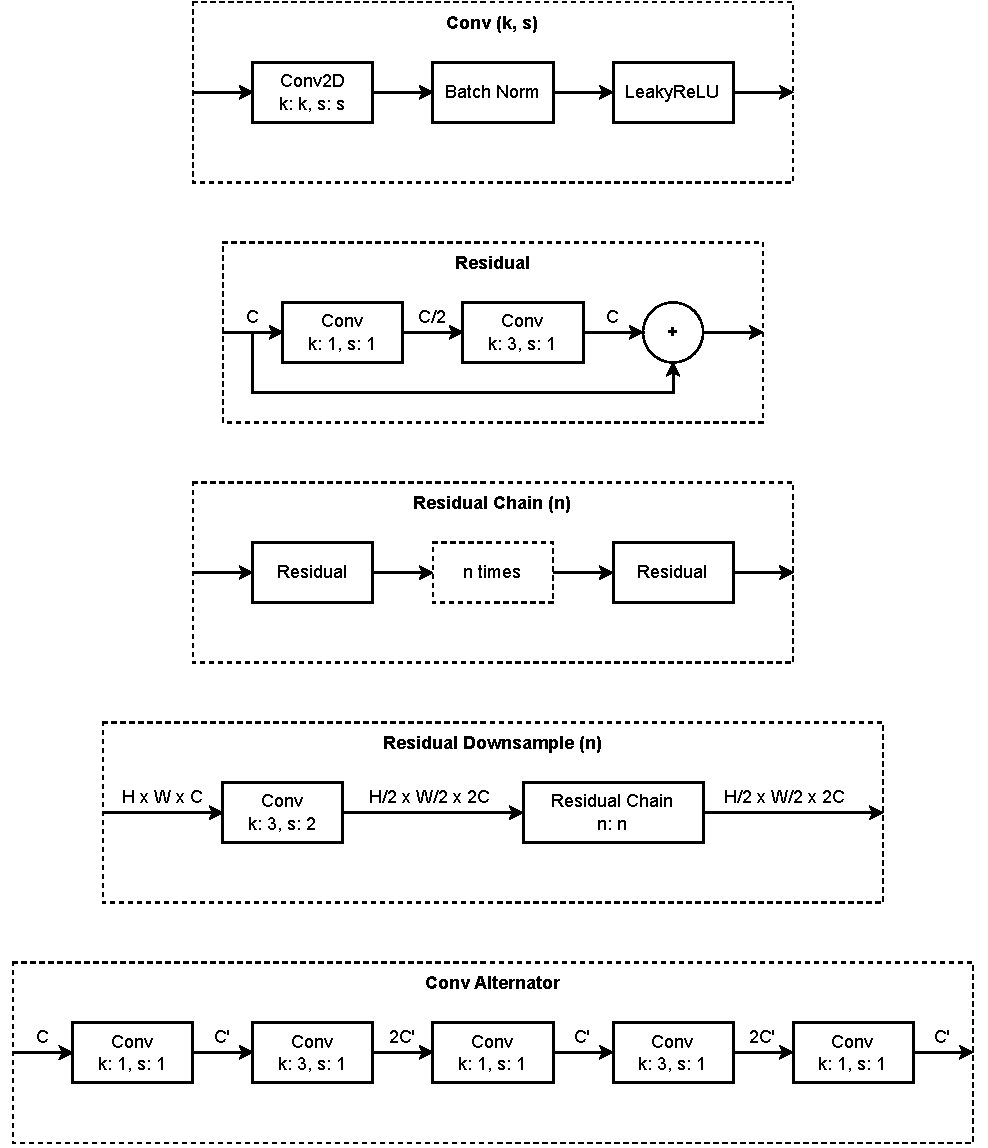
\includegraphics[width=0.75\linewidth]{helpers}
    \caption{Bloki składowe modelu}
    \label{fig:helpers}
\end{figure}

\begin{figure}[!h]
    \centering 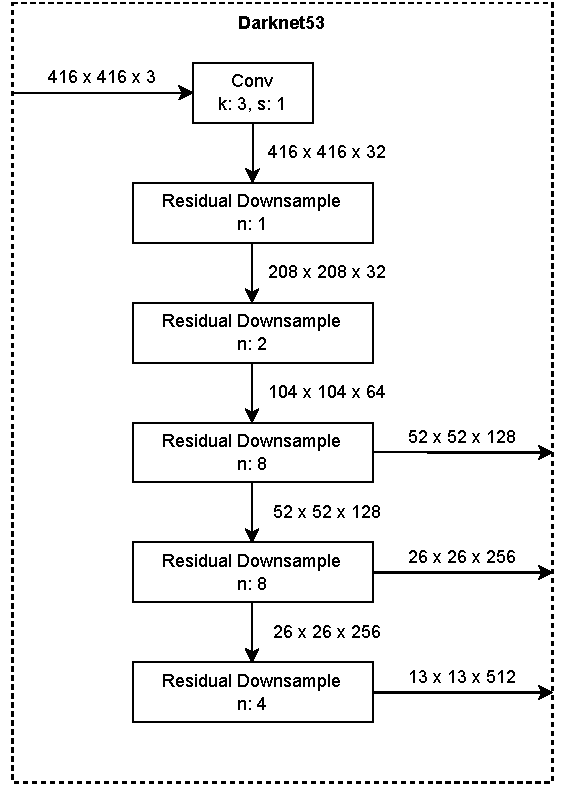
\includegraphics[width=0.5\linewidth]{darknet}
    \caption{Diagram architektury kręgosłupa Darknet53 modelu YOLOv3}
    \label{fig:darknet}
\end{figure}

\begin{figure}[!h]
    \centering 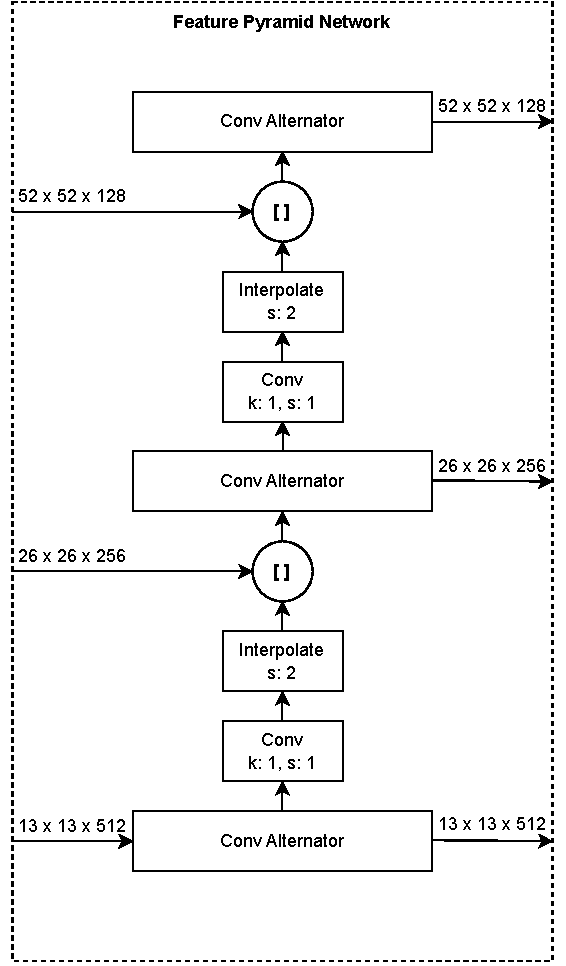
\includegraphics[width=0.55\linewidth]{fpn}
    \caption{Diagram architektury szyjki FPN modelu YOLOv3}
    \label{fig:fpn}
\end{figure}

\begin{figure}[!h]
    \centering 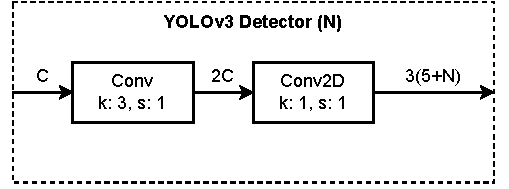
\includegraphics[width=0.45\linewidth]{detector}
    \caption{Diagram architektury głowicy detekcyjnej modelu YOLOv3}
    \label{fig:detector}
\end{figure}

\begin{figure}[!h]
    \centering 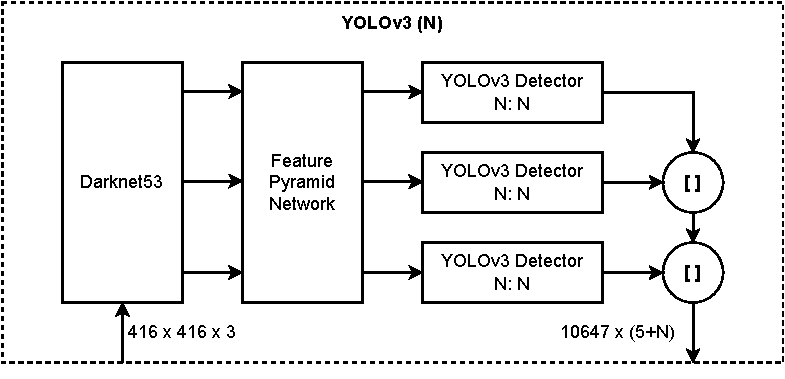
\includegraphics[width=0.65\linewidth]{yolov3}
    \caption{Diagram architektury modelu detekcji obiektów YOLOv3}
    \label{fig:yolov3}
\end{figure}

\FloatBarrier

\subsection{Wyjście z modelu}

Nieprzetworzone wyjście z modelu (predykcje detektora) składa się z trzech zestawów siatek o różnej skali detekcji. Każda komórka siatki zawiera trzy wektory (dla trzech różnych rozmiarów ramek kotwicznych) oznaczające wykryte ramki okalające. Zastosowanie kilku rozmiarów kotwic pozwala na wykrycie kilku obiektów o środku w zbliżonych punktach. W szczególności mogą być to obiektu o różnych proporcjach (np. jeden wydłużony w pionie, drugi w~poziomie).

Pojedyncza ramka okalająca ma postać wektora o wymiarze \(4+1+N\), gdzie cztery pierwsze wymiary opisują pozycję środka ramki (x, y) oraz jej wymiary (szerokość, wysokość), piąty to stopień pewności co do obecności obiektu w~danym miejscu (tzw. \textit{objectness}), natomiast pozostałe \(N\) wymiarów opisuje pewność dla każdej z \(N\) klas.

\subsubsection{Przetwarzanie wyjścia}

Dla wybranego rozmiaru wejścia model YOLOv3 zwraca zawsze stałą liczbę ramek okalających: \((52\cdot52 + 26\cdot26 + 13\cdot13)\cdot3 = 10647\). Aby możliwe było np. zaznaczenie na źródłowym obrazie wykrytych obiektów, konieczne jest pozbycie się nadmiarowych informacji.

Ramki ze wszystkich trzech skali łączone są w jedną listę, a następnie:

\begin{enumerate}
    \item odsiewane są ramki o wartości \textit{objectness} poniżej progu,
    \item spośród nakładających się na siebie ramek wybierane są te o największej pewności (algorytm \textit{Non-maximum Suppression}),
    \item nakładające się na siebie ramki tej samej klasy są scalane ze sobą za pomocą średniej ważonej.
\end{enumerate}

\subsection{Funkcja straty}

Funkcja straty YOLOv3 stanowi sumę następujących składników:

\begin{itemize}
    \item błędu średniokwadratowego pozycji i rozmiarów ramek (tylko dla wykrytych obiektów -- powyżej określonego progu \textit{objectness}),
    \item binarnej entropii skrośnej stopnia pewności wykrycia obiektu,
    \item binarnej entropii skrośnej pewności poszczególnych klas (również tylko dla wykrytych obiektów).
\end{itemize}

Widać zatem, że bierze pod uwagę wszystkie trzy elementy nieprzetworzonego wyjścia z modelu.

Aby obliczyć wartość straty, konieczne jest dostarczenie wartości docelowych wygenerowanych na podstawie etykiet. W uproszczeniu jest to procedura odwrotna do przetwarzania wyjścia z modelu w procesie predykcji.

\section{Usprawnienia}
\label{sec:others}

\subsection{Dopasowanie \textit{anchor boxów} do zbioru danych}

Jedną z metod polepszenia jakości detekcji YOLOv3 jest dostosowanie wielkości ramek kotwicznych do danych, na których model działa. W tym celu należy przetworzyć rozmiary ramek okalających z etykiet używanego zbioru danych algorytmem k-średnich (dla \(k=9\)). Uporządkowane punkty stanowią nowy zestaw kotwic dla modelu. Należy pamiętać, że najmniejsze \textit{anchory} przeznaczone są dla detektora z największą rozdzielczością (który najlepiej wykrywa małe obiekty).

Wyznaczone przez nas \textit{anchor boxy} dla zbioru PKLot (rysunek \ref{fig:clustered_anchors}) wylistowane są poniżej:

\begin{enumerate}
    \item 12x14, 13x17, 15x15,
    \item 17x19, 23x20, 27x25,
    \item 30x15, 38x21, 48x36.
\end{enumerate}

\begin{figure}[!h]
    \centering 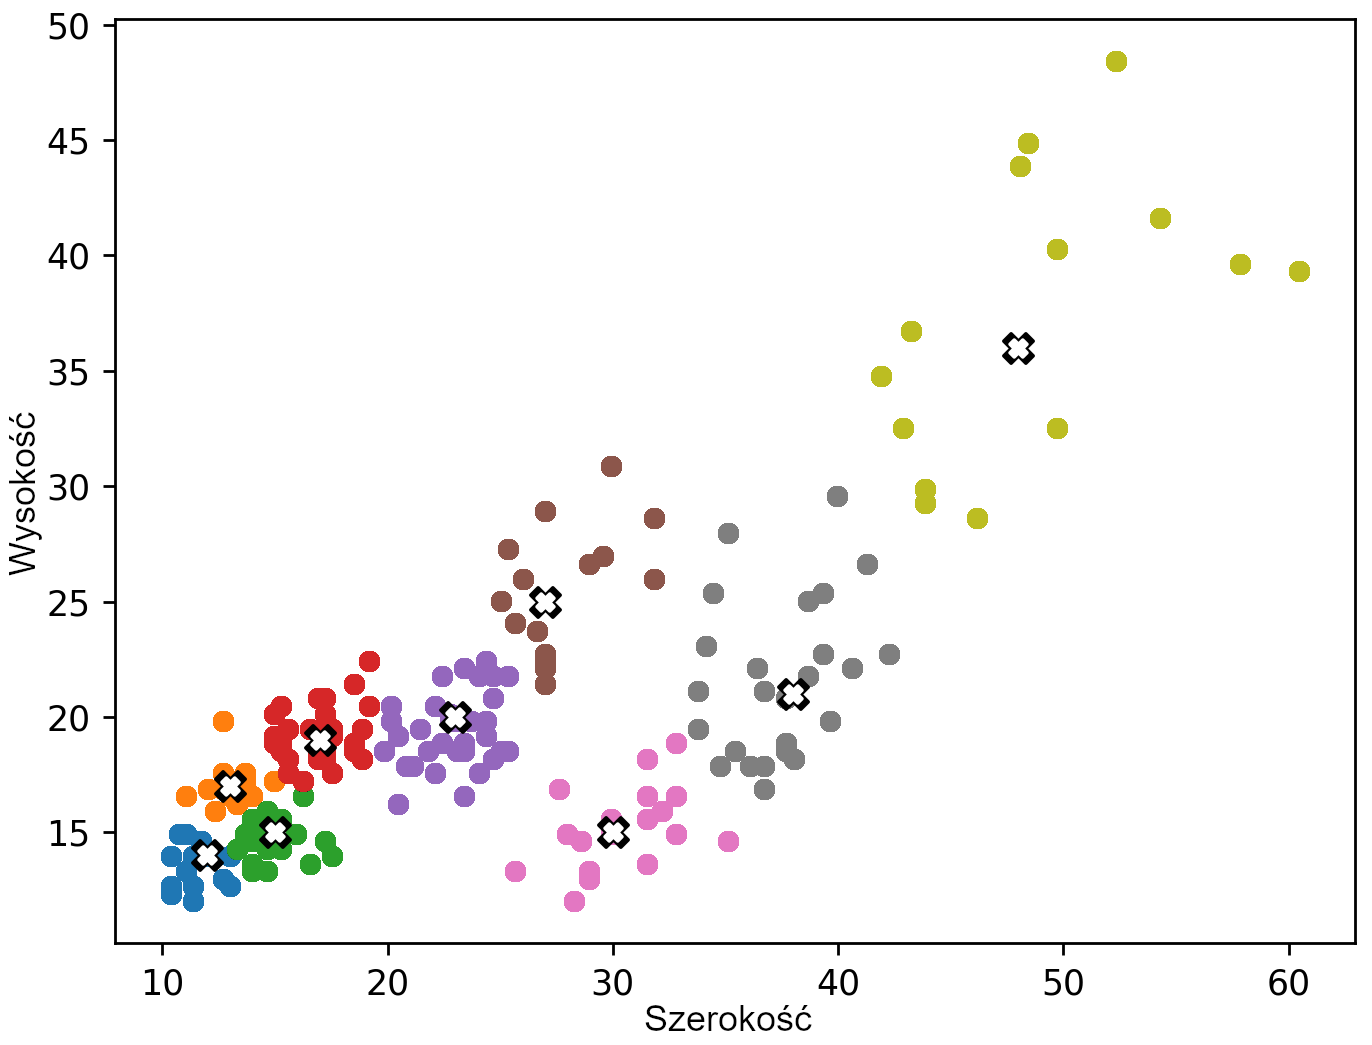
\includegraphics[width=0.65\linewidth]{clustered_anchors}
    \caption{Wizualizacja wyniku klasteryzacji przeprowadzonej na rozmiarach ramek okalających zbioru PKLot}
    \label{fig:clustered_anchors}
\end{figure}

\FloatBarrier

\subsection{Szyjka PANet}

W celu poprawienia jakości sieci, szyjka modelu została wyposażona w~dodatkowa warstwę \textit{Path Aggregation Network} (PANet) pomiędzy oryginalną szyjką (FPN) a detektorami. Miała ona stworzyć tzw. skrót (\textit{shortcut}), czyli potencjalnie krótszą ścieżkę pomiędzy oryginalnym obrazem a głowicą detektora, co pozwala na lepsze określenie położenia obiektu. Warstwa została stworzona na podstawie opisującej ją pracy \citep{liu2018path}. Architektura warstwy przedstawiona jest na rysunku \ref{fig:panet}.

Podczas implementacji planowaliśmy sugerować się implementacją YOLOv4 opisaną w \citep{bochkovskiy2020yolov4}. Model okazał się być silnie dostosowany do problemu i momentami odbiegał od konwencji, dlatego zrezygnowaliśmy z tego pomysłu na rzecz obecnej, prostszej implementacji.

Finalna postać modelu zaprezentowana jest w formie uproszczonej na rysunku \ref{fig:simple_yolov3_panet} i w formie pełnej na rysunku \ref{fig:yolov3_panet}.

\begin{figure}[!h]
    \centering 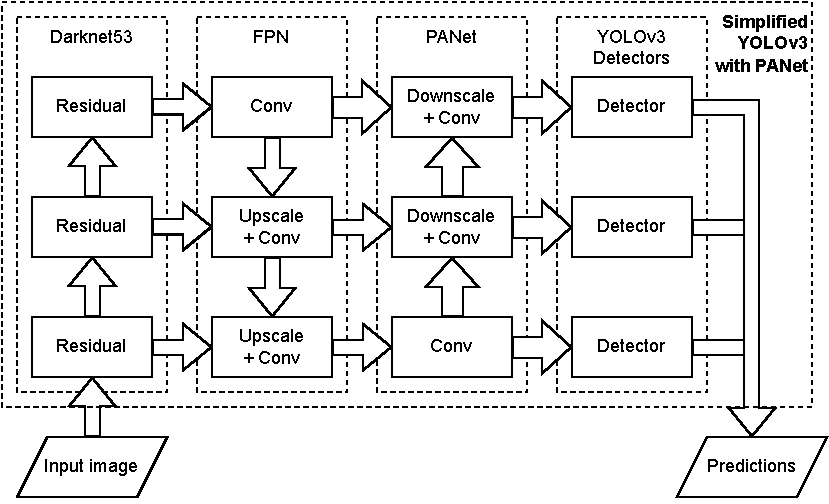
\includegraphics[width=0.65\linewidth]{simple-yolov3-panet}
    \caption{Bardzo uproszczony diagram architektury modelu detekcji obiektów YOLOv3 z dołożoną szyjką PANet}
    \label{fig:simple_yolov3_panet}
\end{figure}

\begin{figure}[!h]
    \centering 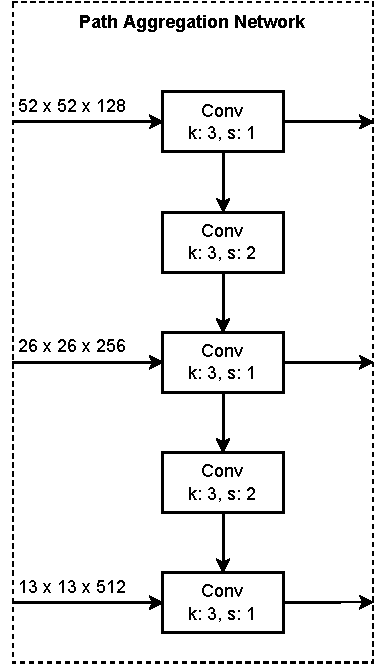
\includegraphics[width=0.35\linewidth]{panet}
    \caption{Diagram architektury szyjki PANet}
    \label{fig:panet}
\end{figure}

\begin{figure}[!h]
    \centering 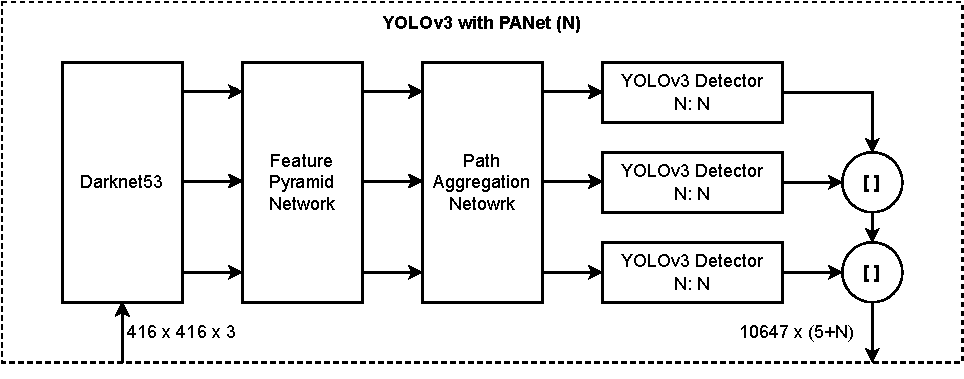
\includegraphics[width=0.7\linewidth]{yolov3-panet}
    \caption{Diagram architektury modelu detekcji obiektów YOLOv3 z dołożoną szyjką PANet}
    \label{fig:yolov3_panet}
\end{figure}

\FloatBarrier

\section{Wyniki}

Tabela \ref{tab:results} prezentuje wyniki uzyskane dla:

\begin{enumerate}
    \item podstawowej implementacji (model \textit{Baseline}) trenowanej przez 85 epok,
    \item implementacji z wyznaczonymi dla zbioru danych kotwicami (model \textit{Anchors}) trenowanej przez 84 epoki,
    \item implementacji z szyjką PANet (model \textit{PANet}) trenowanej przez 57 epok (liczba epok była mniejsza ze względu na dłuższy czas uczenia większego modelu).
\end{enumerate}

\begin{table}
	\caption{Wyniki testów wyuczonego modelu YOLOv3}
	\centering
	\begin{tabular}{llll}
		\toprule
		& \multicolumn{3}{c}{Model}                   \\
		\cmidrule(r){2-4}
            Metryka & Baseline & Anchors & PANet \\
		\midrule
		\(mAP_{@0.5}\)      & 0.94 & 0.94 & 0.94 \\
		\(mAP_{@0.75}\)     & 0.94 & 0.94 & 0.94 \\
		\(mAP_{@0.5:0.95}\) & 0.84 & 0.85 & 0.85 \\
		\bottomrule
	\end{tabular}
	\label{tab:results}
\end{table}

\FloatBarrier

\subsection{Porównanie modeli w czasie}

Ponieważ finalne wyniki (po długotrwałym uczeniu) są zbliżone do siebie, poniżej przedstawiamy wykresy wartości mAP na przestrzeni kolejnych epok.

\begin{itemize}
    \item Kolor szary - model \textit{Baseline}
    \item Kolor zielony - model \textit{Anchors}
    \item Kolor czerwony - model \textit{PANet}
\end{itemize}

\begin{figure}[!h]
    \centering 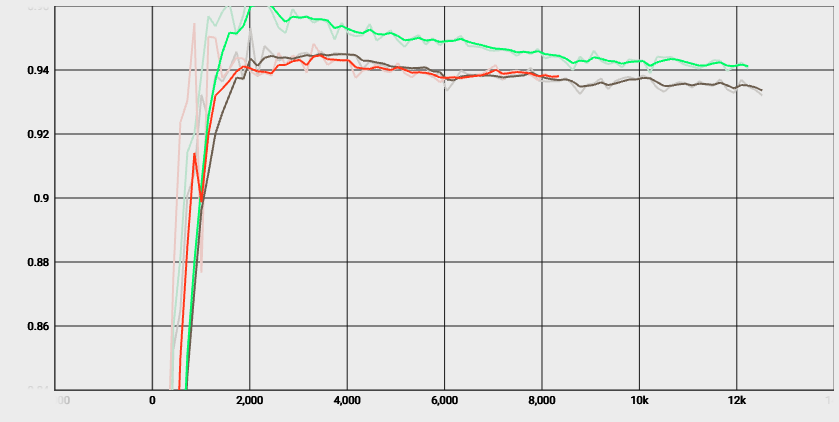
\includegraphics[width=1\linewidth]{map_0_5}
    \caption{Wykres $mAP_{@0.5}$ od ilości obrazów uczących}
    \label{fig:map_0_5}
\end{figure}

\begin{figure}[!h]
    \centering 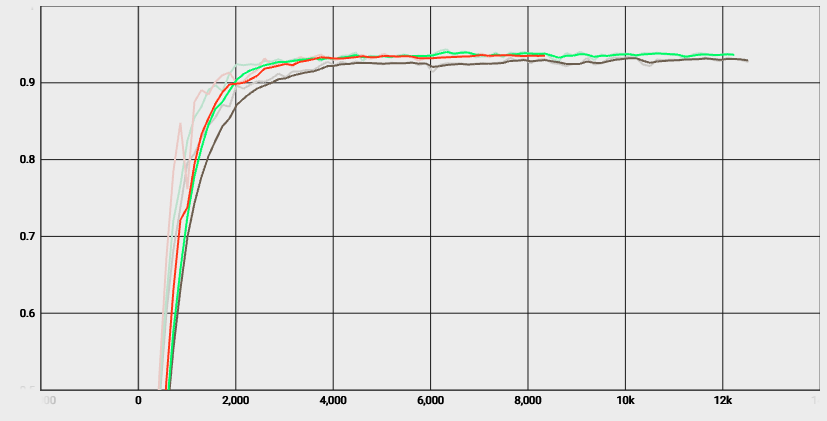
\includegraphics[width=1\linewidth]{map_0_75}
    \caption{Wykres $mAP_{@0.75}$ od ilości obrazów uczących}
    \label{fig:map_0_75}
\end{figure}

\begin{figure}[!h]
    \centering 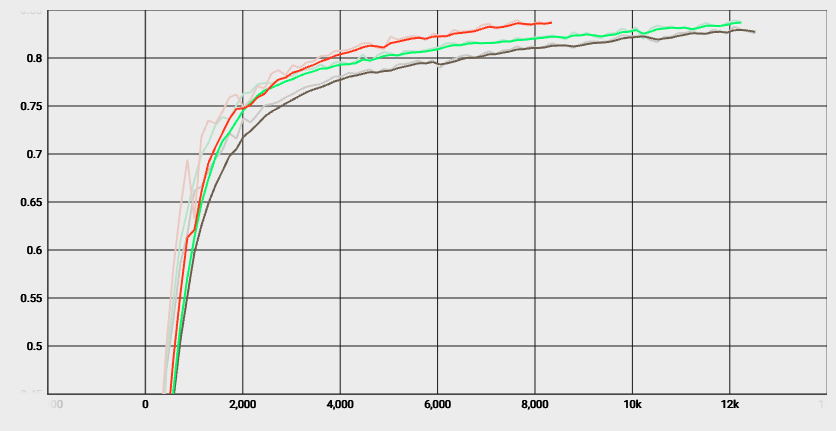
\includegraphics[width=1\linewidth]{map_0_5_0_95}
    \caption{Wykres $mAP_{@0.5:0.95}$ od ilości obrazów uczących}
    \label{fig:map_0_5_0_95}
\end{figure}

\FloatBarrier

\subsection{Wnioski}

\begin{itemize}
    \item Wyniki są bardzo dobre. Niestety, jest duża szansa, że model się przeucza ze względu na niewielką różnorodność danych uczących.
    \item Dostosowanie rozmiarów \textit{anchor boxów} do danych pozwoliło szybciej uzyskać wyższe wartości \(mAP\), ale na dłuższą metę uzyskane wyniki były zbliżone do oryginalnych. Powodem może być wystarczająco dobre dopasowanie oryginalnych rozmiarów kotwic do naszych danych.
    \item Dodanie warstwy PANet spowolniło uczenie pojedynczej epoki modelu, ale znacznie polepszyło wyniki jakie osiąga. Już dla ok. 75\% epok (w porównaniu do innych modeli) uzyskaliśmy wyniki porównywalne do oryginalnego modelu.
    \item Model \textit{Anchors} ma największy przestrzał w $mAP_{@0.5}$ w okolicy 2000 obrazów uczących, a następnie utrzymuje się najwyżej.
    \item Model \textit{PANet} uzyskuje najlepsze wyniki $mAP_{@0.5:0.95}$ zaczynając od 3000 obrazów uczących i stale utrzymuje się nad resztą. Ponieważ jest to powszechnie używana metryka, można powiedzieć, że model ten sprawdza się najlepiej ze wszystkich, które testowaliśmy.
\end{itemize}

\bibliographystyle{unsrtnat}
\bibliography{references}

\end{document}
